\chapter{\sc Geometric Evolution Equations}
\label{ch:geometricpde}

\section[Geometric PDEs]{Geometric PDEs}
As starting point, in order to describe the key ideas of the front tracking
approach, we consider the simple problem of purely geometric evolution
equations. A geometric evolution equation defines the motion of a hypersurface
by prescribing its normal velocity in terms of its geometric quantities. These
problems are part of the more general time-dependent interface evolution
problems category, where the normal velocity depends also on field quantities
evaluated on the analysed hypersurface. A detailed description and analysis can
be found in the review article \cite{DeckelnickDE05}.

Interface evolution problems are everywhere in modern physics and engineering.
Several typical applications can be found in materials science such as the
mathematical modelling of the morphology of microstructure in order to
correctly evaluate the mechanical properties of the material or in void
electro-stress migration where small voids or cracks contained in metallic
materials can change their location and shape according to the presence of
surface diffusion and electro-stress loading. Other typical applications which
can be modelled as time-dependent interface evolution problems are the motion of
grain boundaries which separate differing orientations of the same crystalline
phase, or solid-liquid interfaces exhibiting dendritic structures in
under-cooled solidification. Another research fields where these models can be
applied is image processing to detect the separation of dark regions from a
brighter background and to identify separating contours in order to correctly
cluster the objects in the image. Instead, as explained in Chapter
\ref{ch:introduction}, we apply these techniques to incompressible two-phase
flows problem.

A general geometric evolution equation has the following formulation
\begin{equation}\label{eq:geometric_pde}
\V\,.\,\vec\nu=f(\vec{z}\,,\vec{\nu}\,,\varkappa)
\qquad\mbox{on }\Gamma(t),
\end{equation}
which prescribes the normal velocity $\V\,.\,\vec\nu$ of the
interface $\Gamma(t)$ as a function depending on the position $\vec z$, its
normal direction $\vec{\nu}$ and the sum of its principal curvatures
$\varkappa$. The evolution equation (\ref{eq:geometric_pde}) prescribes only
the normal velocity therefore the overall goal is to find a family of
solutions $\{ \Gamma(t) \}_{t \in [0, T]}$ of closed compact and orientable
hypersurfaces in $\R^{d}$ ($d = 2$ for curves, $d = 3$ for surfaces).

The simplest geometric PDE is the one which arises from motion by mean
curvature,
\begin{equation}\label{eq:mean_curvature}
\V\,.\,\vec\nu=\varkappa\qquad\mbox{on }\Gamma(t).
\end{equation}
This equation describes a surface evolving in such a way that its own normal
velocity is equal to the sum of the $d-1$ principal curvatures of $\Gamma(t)$.

Another important geometric PDE is the one which arises from motion by
surface diffusion
\begin{equation}\label{eq:surface_diff}
\V\,.\,\vec\nu=-\Delta_s \varkappa \qquad\mbox{on }\Gamma(t)\,,
\end{equation}
where we use the Laplace--Beltrami operator $\Delta_s$ defined by
(\ref{eq:surface_laplacian}). In this case the surface normal velocity matches
the surface Laplacian of the mean curvature.

For both models, (\ref{eq:mean_curvature}) and (\ref{eq:surface_diff}), it is
necessary to prescribe the initial interface $\Gamma(0)=\Gamma_0$ in order to
have a well posed problem.

\section[Geometric Analysis]{Geometric analysis}
The aim of this section is to collect some useful definitions and results from
differential geometry. Again we refer to \cite{DeckelnickDE05} which cover the
subject in depth.

A subset $\Gamma \subset \R^d$ is called a $C^2$-hypersurface if for each point
$\vec z_0 \in \Gamma$ there exists an open set $G \subset \R^d$ containing
$\vec z_0$ and a function $g \in C^2(G)$ such that
\begin{equation}
G \cap \Gamma = \{ \vec z \in G \, | \, g(\vec z) = 0 \}
\qquad \mbox{ and } \qquad \nabla \, G(\vec z) \neq 0\,,
\quad \forall\ \vec z \in G \cap \Gamma \, .
\end{equation}
The tangent space $T_{\vec z} \Gamma$ is then the $(d-1)$-dimensional linear
subspace of $\R^d$ that is orthogonal to $\nabla \, g(\vec z)$. It does not
depend on the particular function $g$ which is chosen to describe $\Gamma$. A
$C^2$-hypersurface $\Gamma \in \R^d$ is called orientable if there exists a
vector-valued function $\vec\nu \in C^1(\Gamma, \R^d)$, i.e.~$\vec\nu \in C^1$
in an open neighbourhood of $\Gamma$, such that $\vec\nu(\vec z) \perp T_{\vec
z} \Gamma$ and $|\vec{\nu}(\vec z)| = 1$ for all $\vec z \in \Gamma$. In what
follows, we shall assume that $\Gamma \subset \R^d$ is an orientable
$C^2$-hypersurface.

In order to prove some property of the surface gradient
(\ref{eq:surface_gradient}), we employ the notation
\begin{equation}
\nabla_s \, g(\vec z) = (\underline{D}_1 g(\vec z), \hdots, \underline{D}_{d}
g(\vec z))
\end{equation}
for the $d$ components of the surface gradient. Since $\nabla_s \, g(\vec z)$
is the orthogonal projection of $\nabla \, g(\vec z)$ onto $T_{\vec z} \Gamma$,
it depends only on the values of $g$ on $\Gamma$. Moreover, from
(\ref{eq:surface_gradient}) follows that
\begin{equation}\label{eq:surface_gradient_comp}
\nabla_s \, g(\vec z) \,.\, \vec{\nu}(\vec z)=0\,, \qquad \vec z \in \Gamma\,.
\end{equation}
Similarly, if $g$ is twice differentiable in an open neighbourhood of
$\Gamma$, the surface Laplacian (\ref{eq:surface_laplacian}) can be written as
\begin{equation}\label{eq:surface_laplacian_comp}
\Delta_s g(\vec z) = \nabla_s\, . \,\nabla_s \, g(\vec z) =
\sum_{i = 1}^d \underline{D}_i \underline{D}_i g(\vec z) \, ,
\qquad \vec z \in \Gamma \, ,
\end{equation}
while, if $\vec g$ is a differentiable vector field, the surface divergence
can be rewritten as
\begin{equation}
\nabla_s \,.\, \vec g(\vec z) = \sum_{j = 1}^{d} \underline{D}_j \vec g_j
(\vec z)\,, \qquad \vec z \in \Gamma\,.
\end{equation}

We assume $\vec{\nu} \in C^1$ in a neighbourhood of $\Gamma$ so that we
may introduce the matrix $\mat H(\vec z)$ with components
\begin{equation}\label{eq:matrixHjk}
[\mat H (\vec z)]_{jk} = - \underline{D}_j \nu_k (\vec z)\,, \qquad \vec z \in
\Gamma \, ,
\end{equation}
with $1\leq j,k\leq n$. It can be shown that $\mat H(\vec z)$ is symmetric.
Furthermore,
\begin{equation}
\sum_{k = 1}^{d} [\mat H(\vec z)]_{jk} \nu_k (\vec z) =
\sum_{k = 1}^{d} - \underline{D}_j \nu_k (\vec z) \nu_k (\vec z) =
- \tfrac{1}{2} \underline{D}_j |\vec{\nu}|^2 (\vec z) = 0 \, ,
\end{equation}
since $|\vec{\nu}| = 1$ on $\Gamma$. Thus, $\mat H(\vec z)$ has one
eigenvalue which is equal to zero with corresponding eigenvector
$\vec\nu(\vec z)$. The remaining $d - 1$ eigenvalues $\varkappa_1 (\vec z),
\hdots, \varkappa_{d - 1} (\vec z)$ are called the principal curvatures of
$\Gamma$ at the point $\vec z$. The mean curvature of $\Gamma$ at $\vec z$
can then be defined as the trace of the matrix $\mat H(\vec z)$, that is
\begin{equation}\label{eq:definitionMC}
\varkappa (\vec z) = \sum_{j = 1}^{d} [\mat H(\vec z)]_{jj} = \sum_{j = 1}^{d -
1} \varkappa_j (\vec z) \,.
\end{equation}
Note that (\ref{eq:definitionMC}) differs from the more common
definition of mean curvature,
$\varkappa = \frac{1}{d - 1} \sum_{j = 1}^{d - 1} \varkappa_j$.
From (\ref{eq:matrixHjk}) we derive the following expression for mean
curvature:
\begin{equation}\label{eq:definition2MC}
\varkappa (\vec z)=-\nabla_s \,.\, \vec{\nu}(\vec z) \qquad \vec z \in \Gamma\,.
\end{equation}
In particular, if $\Gamma$ is the unite sphere,
$\Gamma = \{ \vec z \in \R^d : |\vec z| = 1 \}$,
and the unit normal field is chosen to point away from $\Gamma$,
i.e.~$\vec\nu(\vec z) = \vec z$, we obtain that $\varkappa = -
(d - 1)$, on considering the particular function $g(\vec z) = z_j$, $j \in \{
1, \hdots, d \}$ and observing that $\underline{D}_i z_j = \delta_{ij} - \nu_j
\nu_i$. This shows that the mean curvature $\varkappa$ is positive if $\Gamma$
is curved in the direction of the normal.

Moreover, while the sign of $\varkappa$ depends on the choice of the normal
$\vec\nu$, the mean curvature vector $\varkappa \vec\nu$ is an invariant. By
choosing again the particular function $g(\vec z) = z_j$, $j \in \{ 1,
\hdots, d \}$ in (\ref{eq:surface_laplacian_comp}) and recalling the application
of the Laplace-Beltrami operator to each independent variable $z_j$, we deduce
that
\begin{equation}
\Delta_s z_j = - \sum_{i = 1}^{d} \underline{D}_i (\nu_j \nu_i) =
- (\nabla_s \,.\, \vec\nu) \nu_j - \nabla_s \, \nu_j \,.\, \vec\nu = \varkappa
\nu_j\, ,
\end{equation}
which leads to the identity
\begin{equation} \label{eq:LBop}
\Delta_s\, \vec \id = \varkappa\, \vec\nu \qquad \mbox{on $\Gamma(t)$}\,.
\end{equation}
This identity of differential geometry will be useful at a later stage to
obtain a weak formulation of the surface diffusion and mean curvature problems.

\section[Properties of geometric flows]{Properties of geometric flows}
Here we report some fundamental properties of the mean curvature flow and
surface diffusion. In order to derive these properties, we need a transport
theorem for integrals. Consider a family $\{ \Gamma(t) \}_{t \in [0, T]}$
of hypersurfaces that evolve over time. Such a family is called a
$C^{2,1}$-family of hypersurfaces if, for each point $(\vec z_0, t_0) \in
\R^{d} \times (0, T)$ with $\vec z_0 \in \Gamma_0$, there exists an
open set $G \subset \R^{d}$, $\delta > 0$ and a function
$g \in C^{2,1}(G \times (t_0 - \delta, t_0 + \delta))$ such that
\begin{equation}
G \cap \Gamma (t) = \{ \vec{z} \in G \, | \, g (\vec z, t) = 0 \}
\qquad \mbox{ and } \qquad \nabla \, g (\vec z, t) \neq 0
\quad \forall\ \vec z \in G \cap \Gamma(t) \, .
\end{equation}

Now take a family $\{ \Gamma(t) \}_{t \in [0, T]}$ of evolving hypersurfaces
which satisfies the above assumptions and, moreover, suppose that each surface
$\Gamma(t)$ is compact. We are interested in the time derivative of certain
volume and area integrals. As usual, $\surfvol$ is the $(d-1)$-dimensional
Hausdorff measure and $\vol$ is the Lebesgue measure in $\R^d$.

\begin{lemma}
Let $g \in C^1(Q)$, where $Q$ is an open set containing

\begin{equation}
\bigcup_{0 < t < T} \Gamma(t) \times \{ t \} \, .
\end{equation}

Suppose in addition that each surface $\Gamma(t)$ is the boundary of an open
bounded subset $\Omega(t) \subset \R^{d}$. Then

\begin{align}
\ddt \int_{\Omega(t)} g \, \dL{d} & =
\int_{\Omega(t)} \frac{\partial g}{\partial t} \, \dL{d}
+ \int_{\Gamma(t)} g \,\V\,.\,\vec\nu \, \dH{d-1} \, ,
\label{eq:variationVolume} \\
\ddt \int_{\Gamma(t)} g \, \dH{d-1} & =
\int_{\Gamma(t)} \frac{\partial g}{\partial t} \, \dH{d-1} -
\int_{\Gamma(t)} g \, \V\,.\,\vec\nu \varkappa \, \dH{d-1}
\nonumber \\
& + \int_{\Gamma(t)} \frac{\partial g}{\partial \vec{\nu}}\,
\V\,.\,\vec\nu \, \dH{d-1} \, .
\label{eq:variationLength}
\end{align}
\end{lemma}

\begin{proof}
For a proof, see \cite[\S~2.6, Lemma 2.1]{DeckelnickDE05}.
\end{proof}

The evolution of an hypersurface subject to the mean curvature flow
(\ref{eq:mean_curvature}) exhibits the interesting area-decreasing property,
which is obtained from the following lemma.

\begin{lemma}
Let $\Gamma(t)$ be a family of evolving hypersurfaces
satisfying \eqref{eq:mean_curvature} and assume that each $\Gamma(t)$ is
compact. Then

\begin{equation}
\int_{\Gamma(t)} (\V\,.\,\vec\nu)^2 \, \dH{d-1} +
\ddt \surfvol(\Gamma(t)) = 0 \, . \label{eq:lengthDecrease}
\end{equation}

\end{lemma}

\begin{proof}
Choosing $g \equiv 1$ in (\ref{eq:variationLength}) and the evolution law
(\ref{eq:mean_curvature}) yields the desired result.
\end{proof}
The case $d = 2$ is usually referred to as curve shortening flow.

On the other hand, the evolution of an hypersurface subject to surface
diffusion (\ref{eq:surface_diff}) conserves, for closed hypersurfaces, the
enclosed volume and decreases the area as obtained from the following
lemma

\begin{lemma}
Let $\Gamma(t)$ be a family of evolving hypersurfaces
satisfying \eqref{eq:surface_diff} and assume that each $\Gamma(t)$ is
compact and closed. Then
\begin{align}
\ddt \vol(\Omega(t)) & = 0 \,, \label{eq:conservationVolume} \\
\ddt \surfvol (\Gamma(t)) & \leq 0 \,.\label{eq:areaDecrease}
\end{align}
\end{lemma}

\begin{proof}
For (\ref{eq:conservationVolume}), choosing $g \equiv 1$ in
(\ref{eq:variationVolume}) and the evolution law (\ref{eq:surface_diff}) yields
to
\begin{align*}
\ddt \vol(\Omega(t)) &= - \int_{\Gamma(t)} \V\,.\,\vec\nu \,
\dH{d-1} = \nonumber \\
\int_{\Gamma(t)} \Delta_s \, \varkappa \, \dH{d-1} &= - \int_{\Gamma(t)}
\nabla_s \, \varkappa \,.\, \nabla_s \, 1 \, \dH{d-1}= 0 \,.
\end{align*}

Similarly For (\ref{eq:areaDecrease}), choosing $g \equiv 1$ in
(\ref{eq:variationLength}) and the evolution law (\ref{eq:surface_diff}) yields
to
\begin{equation*}
\ddt \surfvol(\Gamma(t)) = - \int_{\Gamma(t)} \V\,.\,\vec\nu
\varkappa \, \dH{d-1} = - \int_{\Gamma(t)} |\nabs \, \varkappa|^2 \, \dH{d-1}
\leq 0 \,.
\end{equation*}
\end{proof}

From a physical point of view, equation (\ref{eq:lengthDecrease}) and
(\ref{eq:areaDecrease}) are associated to the minimization of the surface
energy with constant energy density 1 which is defined as
\begin{equation}\label{eq:surface_energy}
E(\Gamma(t)) = \int_{\Gamma(t)} 1 \, \dH{d-1} \, .
\end{equation}

\section[Front tracking approach]{Front tracking approach}
We always treat the interface using a front tracking approach which involves
seeking a parametrization of the unknown interface over a reference manifold.
More formally, we assume that $(\Gamma(t))_{t\in [0,T]}$ is a sufficiently
smooth evolving hypersurface without boundary which is parametrized by
$\vec x(\cdot,t):\Upsilon\to\R^d$, where $\Upsilon\subset \R^d$ is a given
reference manifold of the same topological type of the evolving hypersurface
$\Gamma(t)$, therefore
\begin{equation}\label{eq:interface_parametrization}
\Gamma(t) = \vec x(\Upsilon,t)\,.
\end{equation}
The position vector $\vec x(\cdot,t)$, for every time $t$, maps a certain point
$\vec{q}$ of the reference manifold $\Upsilon$ to its actual position
$\vec{z}$ on $\Gamma(t)$. Therefore, from (\ref{eq:interface_parametrization}),
we can define the velocity $\V$ of $\Gamma(t)$ as
\begin{equation} \label{eq:V}
\V(\vec z, t) := \vec x_t(\vec q, t) \qquad
\forall\ \vec z = \vec x(\vec q,t) \in \Gamma(t)\,.
\end{equation}

The position vector $\vec x(\cdot,t)$ is one unknown of the problem and, once
computed, the evolution of $\Gamma(t)$ is fully determined. Moreover, all the
geometrical quantities of the hypersurface, e.g. curvature, can be expressed as
derivatives of the parametrization.

It is worth to notice that, at discrete level, the reference manifold
$\Upsilon$ is never used. Indeed, instead of computing the position vector
$\vec x(\cdot,t)$, the unknown variable is the displacement that the previous
discrete interface is subject to. This can be viewed as setting, at every time
step, a new reference manifold which correspond to the actual hypersurface
configuration.

\section[Finite element discretization]{Finite element discretization}
The finite element discretization which we use is based on the seminal paper
\cite{Dziuk91} and we refer to the ones described in
\cite{triplej,triplejMC,gflows3d}. We use a different notation in order to be
consistent with \cite{spurious} and \cite{stokesfitted}.

Putting together the mean curvature flow (\ref{eq:mean_curvature}) with the
identity (\ref{eq:LBop}) we obtain the following system of PDEs
\begin{subequations}
\begin{align}
&\vec{x}_t\,.\,\vec{\nu}=\varkappa\,,\label{eq:mean_curvature_a}\\
&\varkappa\,\vec{\nu}=\Delta_s\,\vec{x}\,,\label{eq:mean_curvature_b}
\end{align}
\end{subequations}
where we have used (\ref{eq:V}) from the front tracking approach in order to
describe the hypersurface velocity $\V$.

Analogously, the surface diffusion problem (\ref{eq:surface_diff}) can be
rewritten as a system of second order equations
\begin{subequations}
\begin{align}
&\vec{x}_t\,.\,\vec{\nu}=-\Delta_s\,\varkappa\,,\label{eq:surf_diff_a}\\
&\varkappa\,\vec{\nu}=\Delta_s\,\vec{x}\,.\label{eq:surf_diff_b}
\end{align}
\end{subequations}
In both problems (\ref{eq:mean_curvature_a}--b) and (\ref{eq:surf_diff_a}--b)
we impose the initial condition $\Gamma(0)=\Gamma_0$.

We consider the partitioning  $0= t_0 < t_1 < \ldots < t_{M-1} < t_M = T$ of
$[0,T]$ into possibly variable time steps
$\tau_m := t_{m+1}-t_m$, $m=0,\ldots, M-1$.

In order to define the parametric finite element spaces on $\Gamma^m$, we
assume that $\Gamma^m=\bigcup_{j=1}^{J_\Gamma} \overline{\sigma^m_j}$, where
$\{\sigma^m_j\}_{j=1}^{J_\Gamma}$ is a family of mutually disjoint open
$(d-1)$-simplices with vertices $\{\vec{q}^m_k\}_{k=1}^{K_\Gamma}$. We also
define the function space
\begin{equation}
\Vh := \{\vec\chi \in [C(\Gamma^m)]^d:\vec\chi\!\mid_{\sigma^m_j}
\in \mathcal{P}_1(\sigma^m_j), j=1,\ldots, J_\Gamma\} =: [\Wh]^d\,,
\end{equation}
where $\Wh \subset H^1(\Gamma^m)$ is the space of scalar continuous
piecewise linear functions on $\Gamma^m$, with $\{\chi^m_k\}_{k=1}^{K_\Gamma}$
denoting the standard basis of $\Wh$ and with $\mathcal{P}_k(\sigma^m)$
denoting the space of polynomials of degree $k$ on $\sigma^m$.

The new surface $\Gamma^{m+1}$ is parametrized respect $\Gamma^m$ using a
parametrization $\vec{X}^{m+1} \in \Vh$, so that $\Gamma^{m+1} =
\vec{X}^{m+1}(\Gamma^m)$.

Then the finite element approximation of the mean curvature flow, which is
based on the variational formulation (\ref{eq:mean_curvature_a}--b), is given
as follows. Let $\Gamma^0$ be an approximation to $\Gamma(0)$. For $m=0,\ldots,
M-1$, find $(\vec{X}^{m+1}, \kappa^{m+1}) \in \Vh \times \Wh$
such that
\begin{subequations}
\begin{align}
&\left\langle \frac{\vec{X}^{m + 1} - \vec{X}^{m}}{\tau_m},
\chi\vec{\nu}^m\right\rangle_{\Gamma^m}^h - \left\langle\kappa^{m+1}, \chi
\right\rangle_{\Gamma^m}^h=0\quad \forall\ \chi \in
\Wh\,,\label{eq:fem_mean_curvature_a}\\
&\left\langle\kappa^{m+1}\vec{\nu}^m, \vec{\eta}\right\rangle_{\Gamma^m}^{h} +
\left\langle\nabla_s\vec{X}^{m + 1},
\nabla_s\vec{\eta}\right\rangle_{\Gamma^m}=0\quad \forall\ \vec\eta \in \Vh,
\label{eq:fem_mean_curvature_b}
\end{align}
\end{subequations}
and set $\Gamma^{m+1} = \vec{X}^{m+1}(\Gamma^m)$. We observe that
(\ref{eq:fem_mean_curvature_a}--b) is a linear scheme in that it leads to a
linear system of equations for the unknowns $(\vec{X}^{m+1}, \kappa^{m+1})$ at
each time level. Here $\langle\cdot,\cdot\rangle_{\Gamma^m}$ is the $L^2$ inner
product over the current polyhedral surface
\begin{equation}\label{}
\langle u,v\rangle_{\Gamma^m} =
\int_{\Gamma^m}uv\,\dH{d-1}\,, \qquad\forall u,v \in
L^2(\Gamma^m),
\end{equation}
where $\surfvol$ is the $(d-1)$-dimensional Hausdorff measure, and
similarly for $\vec{u},\vec{v}\in L^2(\Gamma^m,\R^d)$. In addition,
$\langle \cdot,\cdot\rangle_{\Gamma^m}^h$ is a mass lumped inner product with
the vertices of each triangle of the mesh as quadrature points. If $v,w \in
L^\infty(\Gamma^m)$ are piecewise continuous, with possible jumps
across the edges of $\{\sigma_j^m\}_{j=1}^{J_\Gamma}$, we define the mass
lumped inner product $\langle\cdot,\cdot\rangle_{\Gamma^m}^h$ as
\begin{equation} \label{eq:masslump}
\left\langle v, w \right\rangle^h_{\Gamma^m} :=
\tfrac1d \sum_{j=1}^{J_\Gamma} \surfvol(\sigma^m_j)\,
\sum_{k=1}^{d} (v\,w)((\vec{q}^m_{j_k})^-),
\end{equation}
where $\{\vec{q}^m_{j_k}\}_{k=1}^{d}$ are the vertices of $\sigma^m_j$, and
where we define the limit $v((\vec{q}^m_{j_k})^-)
:= \underset{\sigma^m_j\ni \vec{p}\to \vec{q}^m_{j_k}}{\lim}\, v(\vec{p})$. We
naturally extend (\ref{eq:masslump}) to vector valued functions. We notice that
the second term of (\ref{eq:fem_mean_curvature_b}) is indicated as an exact
integration. This is indeed the case because it is the product of two
piecewise constant functions, since they are the gradient of piecewise linear
functions, therefore the mass lumped inner product (\ref{eq:masslump}) is
exact.

Analogously, the finite element approximation for the surface diffusion problem
(\ref{eq:surface_diff}--b) is analogue to the one obtained for the mean
curvature flow with the linear system (\ref{eq:fem_mean_curvature_a}--b)
changed as
\begin{subequations}
\begin{align}
&\left\langle \frac{\vec{X}^{m + 1} - \vec{X}^{m}}{\tau_m},
\chi\vec{\nu}^m\right\rangle_{\Gamma^m}^{h} - \left\langle\nabla_s\kappa^{m+1},
\nabla_s\chi\right\rangle_{\Gamma^m}=0\quad \forall\ \chi \in
\Wh\,,\label{eq:fem_surf_diff_a}\\
&\left\langle\kappa^{m+1}\vec{\nu}^m, \vec{\eta}\right\rangle_{\Gamma^m}^{h} +
\left\langle\nabla_s\vec{X}^{m + 1},
\nabla_s\vec{\eta}\right\rangle_{\Gamma^m}=0\quad \forall\ \vec\eta \in \Vh\,.
\label{eq:fem_surf_diff_b}
\end{align}
\end{subequations}

If $\Gamma^m$ is an hypersurface without self-intersections, then there exist
a unique solution $(\vec{X}^{m+1}, \kappa^{m+1}) \in \Vh \times \Wh$ to the
systems (\ref{eq:fem_mean_curvature_a}--b) and (\ref{eq:fem_surf_diff_a}--b).
See \cite[Theorem~2.1]{gflows3d} for the complete proof. Furthermore,
the schemes (\ref{eq:fem_mean_curvature_a}--b) and
(\ref{eq:fem_surf_diff_a}--b) are unconditionally stable. See
\cite[Theorem~2.3]{triplej} for the case $d = 2$ and to
\cite[Theorem~2.2]{gflows3d} for $d = 3$ for the complete proofs.

As shown in \cite[Remark~2.3]{triplej} and \cite[\S~4]{gflows3d}, the
continuous-in-time semidiscrete versions of the aforementioned finite element
schemes conserve the enclosed volume exactly. It does not appear possible to
prove the conservation of the enclosed volume for the fully discrete scheme
but, from all the numerical simulations performed in this thesis, we
experimentally observe that the enclosed volume is approximately preserved, and
that the volume loss tends to zero as $\tau \rightarrow 0$.

Finally, in \cite[Remark~2.4]{triplej} the authors proved that for $d=2$ the
continuous-in-time semidiscrete version of (\ref{eq:fem_surf_diff_a}--b)
will always equidistribute the vertices provided that they are not locally
parallel. Unfortunately, it does not appear possible to prove it for fully
discrete scheme. Nevertheless, in practice we see that over a number of time
steps, the vertices are moved tangentially so that they will eventually be
equidistributed. Instead in \cite[\S~4]{gflows3d} the case $d=3$ has been
thoroughly investigated showing that the continuous-in-time semidiscrete version
of (\ref{eq:fem_surf_diff_a}--b) guarantees good mesh properties. Again, in
practice, we notice that it is true for the fully discrete scheme.

We want to stress the fact that this equidistribution property is only
achievable because (\ref{eq:mean_curvature}) and (\ref{eq:surface_diff})
prescribe the velocity only in the normal direction while, in the tangential
direction, the mesh vertices are free to move. Moreover, if instead of the mass
lumped inner product (\ref{eq:masslump}) it is used an exact quadrature, an
analogue of the equidistribution properties cannot be established.

\section[Algebraic formulation]{Algebraic formulation}
As regards the mean curvature flow, (\ref{eq:fem_mean_curvature_a}--b), the
corresponding algebraic system of equations can be written as

\begin{equation}\label{eq:algebraic_mean_curvature}
\begin{pmatrix}
M_m & -\,\frac{1}{\tau_m} \, \vec{N}_{m}^{T} \\
\vec{N}_m & \vec{A}_m
\end{pmatrix}
\begin{pmatrix}
\kappa^{m + 1} \\
\delta \vec{X}^{m + 1}
\end{pmatrix}
=
\begin{pmatrix}
0 \\
- \vec{A}_m \, \vec{X}^{m}
\end{pmatrix} ,
\end{equation}
while, for the system of equations describing the surface diffusion,
(\ref{eq:fem_surf_diff_a}--b), the algebraic system is
\begin{equation}\label{eq:algebraic_surf_diff}
\begin{pmatrix}
A_m & - \,\frac{1}{\tau_m}\, \vec{N}_{m}^{T} \\
\vec{N}_m & \vec{A}_m
\end{pmatrix}
\begin{pmatrix}
\kappa^{m + 1} \\
\delta \vec{X}^{m + 1}
\end{pmatrix}
=
\begin{pmatrix}
0 \\
- \vec{A}_m \, \vec{X}^{m}
\end{pmatrix},
\end{equation}
where we define the interface displacement $\delta \vec{X}^{m + 1}=\vec{X}^{m +
1} - \vec{X}^{m}$ and we have used the trivial identity $\vec{A}_m\,\vec{X}^{m
+ 1} = \vec{A}_m\,\vec{X}^{m}+\vec{A}_m\,\delta \vec{X}^{m + 1} $. We can
notice that the only difference between the above systems occurs in the
upper-left entry of the matrix.

The entries of the matrix are defined as
\begin{eqnarray}
\left[ M_m \right]_{kl} & := & \langle \chi_k^m \, , \chi_l^m
\rangle_{\Gamma^m}^h\,,\label{eq:algebraic_entries_a} \\
\left[ \vec{N}_m \right]_{kl} & := & \langle \chi_k^m \, \vec{\nu}^m\,,
\chi_l^m \rangle_{\Gamma^m}^h\,,\label{eq:algebraic_entries_b} \\
\left[ A_m \right]_{kl} & := & \langle \nabla_s \chi_k^m \, , \nabla_s
\chi_l^m \rangle_{\Gamma^m}\,,\label{eq:algebraic_entries_c}
\end{eqnarray}
where $\{\chi_k^m\}$ are the basis functions of the finite element space of
piecewise linear continuous functions $W(\Gamma^m)$ and
\begin{equation}\label{eq:algebraic_entries_d}
[\vec{A}_m]_{kl} := [A_m]_{kl} \mat \id\,.
\end{equation}
We notice that for entries (\ref{eq:algebraic_entries_c}) holds
\begin{equation}
\begin{split}
& \langle \nabla_s \chi_k^m \, , \nabla_s \chi_l^m \rangle_{\Gamma^m} = \langle
\nabla \chi_k^m \, -\,\nabla \chi_k^m\,.\,\vec \nu\,\vec\nu, \nabla
\chi_l^m \, -\,\nabla \chi_l^m\,.\,\vec \nu\,\vec\nu\rangle_{\Gamma^m} = \\
& \langle \nabla \chi_k^m \, , \nabla \chi_l^m \rangle_{\Gamma^m}\,
- 2\, \langle \nabla \chi_k^m \,.\,\vec\nu\,\vec\nu , \nabla \chi_l^m
\rangle_{\Gamma^m}
+\langle \nabla \chi_k^m \,.\,\vec\nu\,\vec\nu , \nabla \chi_l^m
\,.\,\vec\nu\,\vec\nu \rangle_{\Gamma^m} = \\
& \langle \nabla \chi_k^m \, , \nabla \chi_l^m \rangle_{\Gamma^m}
- \langle \nabla \chi_k^m \,.\,\vec\nu\,\vec\nu , \nabla \chi_l^m
\rangle_{\Gamma^m} =
\langle \nabla \chi_k^m \, , \nabla \chi_l^m \rangle_{\Gamma^m}\,,
\end{split}
\end{equation}
where, in the last equality, we have used the fact that $\langle \vec
\nu\,,\,\nabla \chi_k^m  \rangle_{\Gamma^m}$. Therefore, in practice,
(\ref{eq:algebraic_entries_c}) can be assembled as the standard Laplacian
term $\langle \nabla \chi_k^m \, , \nabla \chi_l^m \rangle_{\Gamma^m}$.

The linear systems (\ref{eq:algebraic_mean_curvature}) and
(\ref{eq:algebraic_surf_diff}) are invertible under a suitable assumption on the
triangulation at each time step, see \cite{gflows3d}. The algebraic system
(\ref{eq:algebraic_mean_curvature}) and (\ref{eq:algebraic_surf_diff}) are
very small also for fine meshes therefore they can be solved very efficiently
with a sparse factorization package such as \verb|UMFPACK|, see \cite{Davis04}.

\section[Numerical results]{Numerical results}
Here we report several numerical examples to benchmark the schemes
(\ref{eq:fem_mean_curvature_a}--b) and (\ref{eq:fem_surf_diff_a}--a).

We remark that the initial mean curvature of an hypersurface can be obtained
directly from the identity (\ref{eq:LBop}). Equivalently, the unknown
mean curvature $\varkappa$ can be computed by solving the algebraic system
\begin{equation}\label{eq:algebraic_initial_curvature}
\begin{pmatrix}
0 & -\,\frac{1}{\tau} \, \vec{N}_{0}^{T} \\
\vec{N}_0 & \vec{A}_0
\end{pmatrix}
\begin{pmatrix}
\kappa \\
\delta \vec X
\end{pmatrix}
=
\begin{pmatrix}
0 \\
- \vec{A}_0 \, \vec{X}^{0}
\end{pmatrix}
.
\end{equation}
Indeed, the algebraic system (\ref{eq:algebraic_initial_curvature}) is the
discretization of the stationary geometric PDE
\begin{equation}
\V\,.\,\vec\nu=0\qquad\mbox{on }\Gamma(t)\,,
\end{equation}
coupled with the identity (\ref{eq:LBop}) therefore $\delta\vec X \equiv 0$ and
(\ref{eq:algebraic_initial_curvature}) can be simply rewritten as
\begin{equation}
\vec{N}_0\,\kappa=- \vec{A}_0 \, \vec{X}^{0}\,,
\end{equation}
which is the discrete version of (\ref{eq:LBop}).

\subsection[Mean curvature flow with a sphere as initial condition]
{Mean curvature flow with a sphere as initial condition}
As regards the mean curvature flow, the simplest case is to use a sphere as the
initial condition, see \cite{Ilmanen98}. In this case, the solution to the
geometric evolution equation is known in closed form and it is a shrinking
sphere. Let $\Gamma(t) = \{ \vec z \in \R^d : |\vec z -\vec z_0| = r(t) \}$,
oriented by the outer normal $\vec \nu(\vec{z}) = \frac{\vec z - \vec
z_0}{r(t)}$. It is straightforward to derive that
$\V\,.\,\vec\nu = r^{\prime}(t), \varkappa = - \frac{d -
1}{r(t)}$ on $\Gamma(t)$, so that $\Gamma(t)$ moves by mean curvature provided
that $r^{\prime}(t) = - \frac{d - 1}{r(t)}$. The solution of this separable
variable ODE is easily given by $r(t) = \sqrt{r_0^2 - 2(d - 1)t}, \, 0 \leq t <
t_e$, where $\Gamma(0) = \{ \vec z \in \R^d : |\vec z -\vec z_0| = r_0 \}$ and
$t_e=\frac{r_0^2}{2(d - 1)}$ is the so called extinction time. It is worth
noting that the surface $\Gamma(t)$ shrinks to a point as $t \rightarrow t_e$.

Figure~\ref{fig:mcf_sphere} shows the evolution of a sphere with initial radius
$r_0=5$ at time $t=0$, $t=2$, $t=4$ and $t=6$ respectively. In this case, the
extinction time, is $t_e=6.25$. The number of mesh elements is $J_\Gamma=3026$
and the time step is constant and equal to $\tau=10^{-3}$.

\begin{figure}[htbp]
\centering
\subfloat[$t=0$]{
\includegraphics[width=.45\textwidth]{figures/geometric_pdes/mcf_sphere_0.ps}}
\quad
\subfloat[$t=2$]{
\includegraphics[width=.45\textwidth]{figures/geometric_pdes/mcf_sphere_2.ps}}
\\
\subfloat[$t=4$]{
\includegraphics[width=.45\textwidth]{figures/geometric_pdes/mcf_sphere_4.ps}}
\quad
\subfloat[$t=6$]{
\includegraphics[width=.45\textwidth]{figures/geometric_pdes/mcf_sphere_6.ps}}
\caption[Shrinking sphere experiment]{Surface evolution of a sphere of initial
radius $r_0=5$ subject to mean curvature flow.}
\label{fig:mcf_sphere}
\end{figure}

Figure~\ref{fig:mcf_sphere_radius} shows in red the average radius length
over time of the sphere while the blue plot is the the exact length computed
from the analytical solution.

\begin{figure}[htbp]
\centering
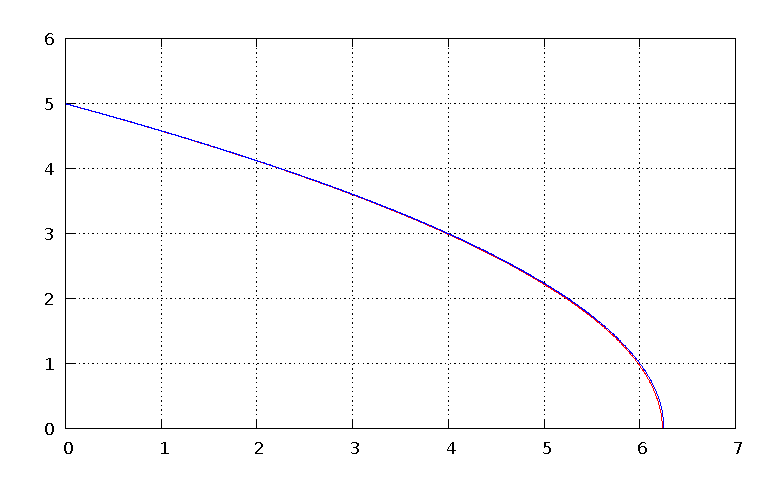
\includegraphics[width=.45\textwidth]
{figures/geometric_pdes/mcf_sphere_radius.ps}
\caption[Shrinking sphere radius]{Average radius of a sphere of initial radius
$r_0=5$ subject to mean curvature flow. In blue the analytical solution while in
red the computed one.}
\label{fig:mcf_sphere_radius}
\end{figure}

\subsection[Equidistribution property]{Equidistribution property}
In order to show the equidistribution property of the scheme, we simulate the
evolution, under surface diffusion, of a circle of radius $r_0=0.5$ with a very
poor initial mesh quality. Indeed, the initial curve consists of a semi-circle
and a single additional node on the periphery of the circle for a total number
of mesh elements equal to $J_\Gamma=32$.

Figure~\ref{fig:sd_circle} shows the mesh evolution at time $t=0$, $t=0.05$,
$t=0.25$ and $t=10$ respectively with a constant time step equal to
$\tau=10^{-2}$. One can clearly see that although the true solution, which is a
circle, is reached very quickly, in the remaining time the vertices are
continually moved tangentially, which results in a further decrease in the ratio
$\frac{\max_{\sigma\in \Gamma^m}(\surfvol(\sigma))}
{\min_{\sigma\in\Gamma^m}(\surfvol(\sigma))}$, which approaches the optimal
value 1. This mesh quality indicator is simply the ratio between the maximum
and minimum segment of the hypersurface.

\begin{figure}[htbp]
\centering
\subfloat[$t=0$]{
\includegraphics[width=.45\textwidth]{figures/geometric_pdes/sd_circle_0.ps}}
\quad
\subfloat[$t=0.05$]{
\includegraphics[width=.45\textwidth]{figures/geometric_pdes/sd_circle_005.ps}}
\\
\subfloat[$t=0.25$]{
\includegraphics[width=.45\textwidth]{figures/geometric_pdes/sd_circle_025.ps}}
\quad
\subfloat[$t=10$]{
\includegraphics[width=.45\textwidth]{figures/geometric_pdes/sd_circle_10.ps}}
\caption[Equidistribution property experiment]{Surface evolution of a circle of
initial radius $r_0=0.5$ subject to surface diffusion.}
\label{fig:sd_circle}
\end{figure}

In Figure~\ref{fig:sd_circle_tau} we see that the equidistribution velocity is
varying inversely with the size of $\tau$. For example, when $\tau=10^{-4}$,
the equidistribution is reached almost instantaneously.

\begin{figure}[htbp]
\centering
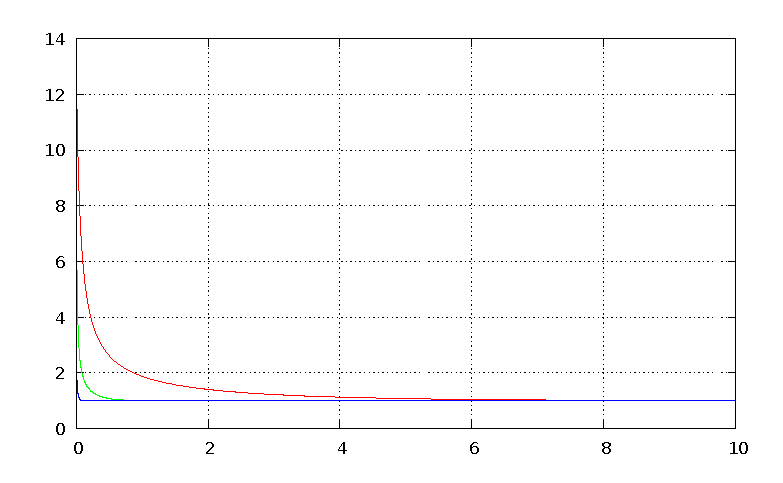
\includegraphics[width=.45\textwidth]
{figures/geometric_pdes/sd_circle_tau.ps}
\caption[Equidistribution velocity]{Time evolution of the ratio
$\frac{\max_{\sigma\in \Gamma^m}(\surfvol(\sigma))}
{\min_{\sigma\in\Gamma^m}(\surfvol(\sigma))}$ for a circle of initial radius
$r_0=0.5$ subject to surface diffusion. In red $\tau=10^{-2}$, in green
$\tau=10^{-3}$ and in blue $\tau=10^{-4}$.}
\label{fig:sd_circle_tau}
\end{figure}

\subsection[Surface diffusion with a cage as initial condition]
{Surface diffusion with a cage as initial condition}
Our last simulation is inspired by the test in \cite[Fig.~15]{gflows3d}. We
investigate the evolution of a cage subject to surface diffusion. The
dimensions of the initial surface are $4 \times 4 \times 4$, with the region
enclosed by $\Gamma(0)$ given as the union of 12 cuboids of dimension $4 \times
1 \times 1$.

Figure~\ref{fig:sd_cage} shows the cage evolution at time $t=0$, $t=0.2$,
$t=0.4$ and $t=0.6$ respectively. The number of mesh elements is
$J_\Gamma=3816$ and the time step is constant and equal to $\tau=10^{-2}$.

\begin{figure}[htbp]
\centering
\subfloat[$t=0$]{
\includegraphics[width=.45\textwidth]{figures/geometric_pdes/sd_cage_0.ps}}
\quad
\subfloat[$t=0.2$]{
\includegraphics[width=.45\textwidth]{figures/geometric_pdes/sd_cage_02.ps}}
\\
\subfloat[$t=0.4$]{
\includegraphics[width=.45\textwidth]{figures/geometric_pdes/sd_cage_04.ps}}
\quad
\subfloat[$t=0.6$]{
\includegraphics[width=.45\textwidth]{figures/geometric_pdes/sd_cage_06.ps}}
\caption[Cage experiment]{Surface evolution of a cage $4 \times 4 \times 4$
subject to surface diffusion.}
\label{fig:sd_cage}
\end{figure}

At time $t=0.6$ a topological change is encountered when the six holes of the
surface are about to close to form a hollow ball.
Figure~\ref{fig:sd_cage_section} shows a section of this hallow ball. A
topological change breaks the front tracking approach since the reference
manifold $\Gamma^m$ is not topological compatible with the unknown surface
$\Gamma^{m+1}$. In practice, it is possible to apply some heuristic algorithms
for the detection of topological changes, such as the merging of surfaces into
one or the pinching-off of one surface from another, which can lead to a
modified surface mesh that can be handled again with the parametric approach.

\begin{figure}[htbp]
\centering
\includegraphics[width=.45\textwidth]
{figures/geometric_pdes/sd_cage_06_section.ps}
\caption[Cage section]{Section at $t=0.6$ of a cage $4 \times 4 \times 4$
subject to surface diffusion.}
\label{fig:sd_cage_section}
\end{figure}

Finally, Figure~\ref{fig:sd_cage_energy} shows the evolution of the surface
energy (\ref{eq:surface_energy}) over time. As expected, see
(\ref{eq:areaDecrease}), this energy is monotonically decreasing.

\begin{figure}[htbp]
\centering
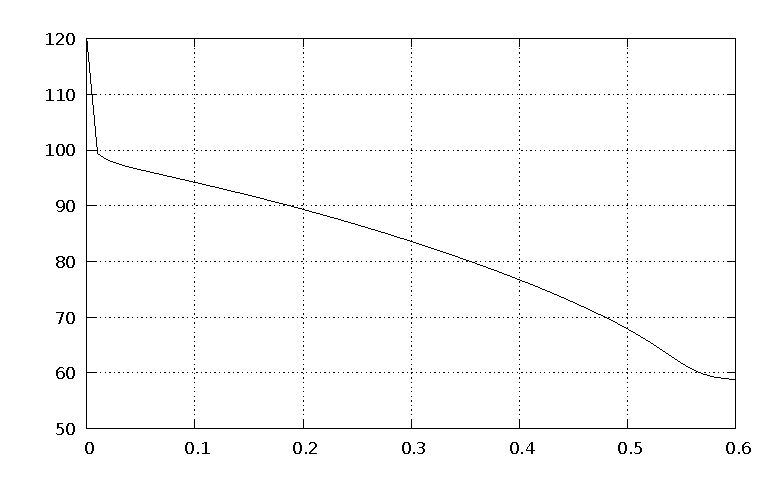
\includegraphics[width=.45\textwidth]
{figures/geometric_pdes/sd_cage_energy.ps}
\caption[Cage surface energy]{Surface energy evolution $\surfvol(\Gamma^m)$ of
a cage $4 \times 4 \times 4$ subject to surface diffusion.}
\label{fig:sd_cage_energy}
\end{figure}
